\section{Phrase Structure Grammar}
\scriptsize{Grammar g} {\tiny <T, NT, S, R>}\\
\scriptsize{Language} {\tiny set of all strings g can generate\\
L(PSG) = \{(the, child, reads, a, book), (a, child, reaeds, the, book), (the, book, reads, a, child), (a, book, reads, the, child)\}}\\
\scriptsize{Rewrite} {\tiny tree notation, rewrite notation and bracket notation are structurally equivalent}\\
\scriptsize{Feature of PSG} {\tiny strongly restrict the number of possible sentences via linearization constraints in the non-terminal rules}\\
\scriptsize{binarization constraint} {\tiny all rewrite rules have only 1 symbol on the left and maximally 2 symbols on the right}\\
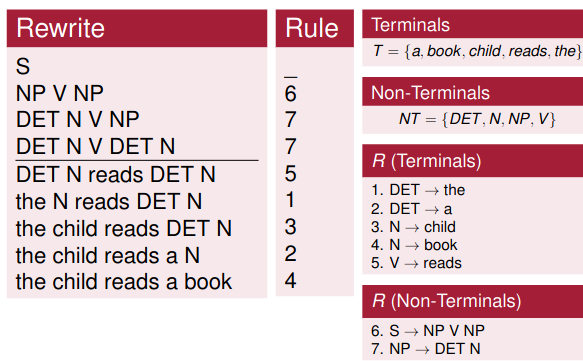
\includegraphics[scale=0.22]{psg.png}\\
\scriptsize{Expanding PSG}
{\tiny vocabulary, morphology}\\
\scriptsize{Problems}
{\tiny complicated agreement systems; implementing morphological features}\\
\scriptsize{verb position}
{\tiny verb-final, verb-medial, verb-initial, transitive, ditransitive (introduction of recursive rule will lead to generation of ungrammatical sentences}\\
\scriptsize{passive}
{\tiny VP -> AUX VP (aux: is), have to formulate different phrase structure rules for active and passive sentences}\\
\scriptsize{Pros}
{\tiny implements linearization constraints exlicitely; grounded on solid mathematical footing (automata theory); can be extended to model morphological features; easily implementable in computational frameworks}\\
\scriptsize{Cons}
{\tiny not all languages need rules (free word order); cumbersome to implement morphological features; excludes semantic aspects from grammaticality; infinite number of PSGs without further constraints}